\clearpage\clearpage
\graphicspath{{sdf/key_management_layer/figures/}}
\acresetall

\section{Key Management Layer}
% Show subsubsections on the Table of Contents
\setcounter{tocdepth}{4}
\setcounter{secnumdepth}{4}

\begin{refsection}
	\begin{tcolorbox}
		\begin{tabular}{p{2.75cm} p{0.2cm} p{10.5cm}}
			\textbf{Goal}          &:& Design and implementation of a quantum key management layer\\
			\textbf{Directory}     &:& sdf/key\_management\_layer\\
			\textbf{Contributors}   &:& Armando Nolasco Pinto (2023/03/-- ----/--/--) \\
									&& Diogo Matos (2023/03/14 - ----/--/--) \\
		\end{tabular}
	\end{tcolorbox}

%%%%%%%%%%%%%%%%%%%%%%%%%%%%%%%%%%%%%%

\subsection{Introduction}

Quantum Key Distribution (QKD) enables the negotiation of cryptographic keys in a secure manner without relying on computational complexity to achieve its security. On top of the QKD systems a \ac{KML} need to exist in order to mediate the key provisioning to the applications. The key manager provides keys with characteristics requested by the apps and bond to a pre-negotiated quality of service. The proposed system follows Discretion's and ETSI standards [1][2][3]. The system differentiates itself in the fact that mostly (or only) receives quantum oblivious keys from the QKD devices. A future version of the key manager should be able to offer classical, post-quantum and quantum keys, helping its integration into existing networks and providing more flexibility to its clients.

%%%%%%%%%%%%%%%%%%%%%%%%%%%%%%%%%%%%%%

\subsection{Notes and considerations}
\begin{itemize}
	\item During this section, quantum oblivious keys will be divided into two types, A and X. In any connection involving a oblivious keys, one of the parties will receive keys of type A and the other of type X. Keys of type A are whole keys, and keys of type X are keys that are a representation, in a oblivious key fashion, of half of its respective type A key.
	\item In this first version, only the quantum part of the system is specified, though it's our intention to support classical and post-quantum keys too. Nevertheless the system from scratch should be modular enough to facilitate this integration. 
	\item This section will be gradually updated even during the implementation of the system. Some dependencies, like the SDN Agent and the QKD Devices, and issues only found during the implementation might trigger the need to change/enrich this specifications. 
\end{itemize}

%%%%%%%%%%%%%%%%%%%%%%%%%%%%%%%%%%%%%%

\subsection{Architecture}

\begin{figure}[H]
	\centering
	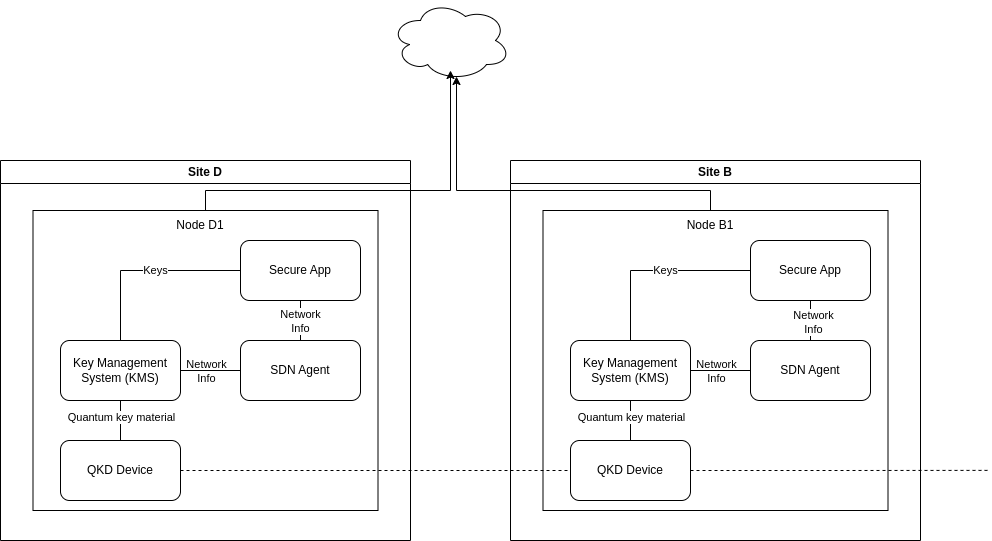
\includegraphics[width=15cm]{kml_arch.png}
	\caption{System architecture}
	\label{fig:kmlarch}
\end{figure}

In the diagram above (\autoref{fig:kmlarch} a simple overview over the whole system in a two node scenario where the \ac{KMS} is integrated can be seen. The dashed line represents a quantum link and the cloud is the black network where, for example, the \ac{SDN} Controller is located. Each secure site have one or more SD-QKD nodes each identified by its \textit{qkdn\_id}. More information on SD-QKD nodes, QKD interfaces, QKD key association links can be found in the standard ETSI QKD 015 [2]. The \ac{KMS} is connected to a physical layer that provides keys to it. These keys can be symmetrical or oblivious and can be generated in distinct manners - classical, post-quantum or quantum (our main focus). Multiple applications are connected to it in order to retrieve keys. Both interfaces, to the applications and to the QKD devices, are based on ETSI QKD 004 standard [1]. Each KMS is connected to at least one KMS that is considered to be its peer since they receive matching keys from the physical layer. Also, the \ac{SDN} agent (\ac{SDN} Controller representative inside the node) is connected to the \ac{KMS} and is used, from the \ac{KMS} perspective, to retrieve information about the network, provide QoS parameters and to receive command orders.

The type of key sources connected to the \ac{KMS} might limit the keys that this one can provide. The connection to a oblivious key source is enough to provide both symmetrical and oblivious keys and even random numbers. Though the key rate might be lower because in order generate a symmetrical key using oblivious keys, twice of the size of wished key will be used.

\begin{figure}[H]
	\centering
	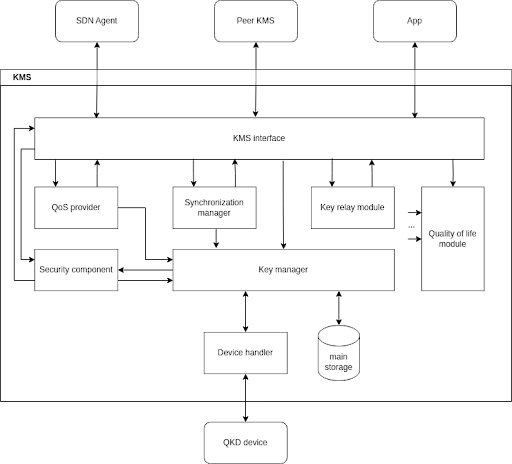
\includegraphics[width=10cm]{kms_modules.png}
	\caption{\ac{KMS} logical modules}
	\label{fig:kmsmodules}
\end{figure}

Apart from just receiving and sending keys through its South and North bound interfaces respectively, the \ac{KMS} need to store, maintain, synchronize, derive and relay (forward) keys. The \ac{KMS} is divided into various logical modules (\autoref{fig:kmsmodules}), namely:

\begin{itemize}
	\item{ \underline{KMS interface (north bound interface)}} 
	
	ETSI QKD 004 based interface to the applications(see \ref{kms_api_apps}). Interface to the \ac{SDN} Agent (to be defined) and to its peer \ac{KMS}s.
	
	\item{\underline{QoS provider}} 
	
	Gathers and provides all QoS parameters to be used to negotiate with the applications and to send them to the \ac{SDN} Agent when requested.
	
	\item{\underline{Synchronization manager}} 
	
	Handles the synchronization protocol (see \ref{key_synch})
	
	\item{\underline{Security component}} 
	
	Implements all cryptographic algorithms used during the operation of the \ac{KMS}.
	
	\item{\underline{Key relay module}} 
	
	Handles the key relay(forwarding) process (see \ref{kms_key_relay}).
	
	\item{\underline{Key manager}} 
	
	Maintains and handles keys. Is mainly used for key material retrieval, storage, etc. It's involved in almost any activity related with keys.
	
	\item{\underline{Base functionality}} 
	
	Handles several quality-of-life features such as logging and configuration.
	
	\item{\underline{Device handler}} 
	
	Handles devices connected to the \ac{KMS} (such as the QKD devices).

\end{itemize}


%%%%%%%%%%%%%%%%%%%%%%%%%%%%%%%%%%%%%%

\subsection{KMS interface to the apps}
\label{kms_api_apps}
This interface follows the ETSI QKD 004 [1] standard in pull mode, it was presented before in \ref{etsi_004} where more detailed information can be found, nevertheless here is made a brief overlook of the API. During the implementation all error cases should be considered and handled has defined in the standard.

\vspace{5mm}

The interaction between \ac{KMS} and app is based on three request, namely:

\begin{lstlisting}
	OPEN_CONNECT(in source, in destination, inout QoS, inout Key_stream_ID, out status)
	GET_KEY(in Key_stream_ID, inout index, out Key_buffer, inout Metadata, out status)
	CLOSE(in Key_stream_ID, out status)
\end{lstlisting}

The OPEN\_CONNECT request is made by an app to create a key stream with the characteristics specified in the QoS field. A \ac{KSID} is returned. If the OPEN\_CONNECT request is made with a value in the Key\_stream\_ID field, it connects to an existing Key Stream instead of creating a new one. 

The GET\_KEY request is used by the apps to retrieve keys. It can be made with or without an index. With a given index, the \ac{KMS} will return the key, if exists, with that index. Otherwise, it return the oldest key that was created by its peer by not retrieved yet, if there is no keys to be return, a new one will be created and returned alongside with its index.

The CLOSE request is used to terminate a Key Stream connection. The peer still can retrieve already created and unexpired keys.

\vspace{5mm}

Since the proposed system is able to offer different types of keys, to the Quality of Service field in the OPEN\_CONNECT was added one extra parameter called 'Key\_type'. After the changes, the QoS parameters are:
		
\begin{itemize}
	\item{\underline{Key\textunderscore type}}
				
	Key type for the key stream. 0: classical symmetrical, 1: P.Q. symmetrical, 2: quantum symmetrical, 3/4: classical oblivious (A/X), 5/6: P.Q. oblivious (A/X), 7/8: quantum oblivious (A/X).
				
	\item{\underline{Key\textunderscore chunk\textunderscore size}}
				
	Length of the key buffer requested by the application. 32 bit unsigned integer.
				
	\item{\underline{Max\textunderscore bps}}
			
	Maximum key rate requested in bits per seconds. 32 bit unsigned integer.
				
	\item{\underline{Min\textunderscore bps}}
			
	Minimum key rate requested in bits per seconds. 32 bit unsigned integer.
				
	\item{\underline{Jitter}}
				
	Maximum expected deviation, in bps, for key delivery. 32 bit unsigned integer.
	
	\item{\underline{Timeout}}	
	
	Time, in msec, after which the all will be aborted, returning an error.
			
	\item{\underline{TTL (Time to Live)}}
			
	Time after which the keys corresponding to this Key\textunderscore stream\textunderscore ID shall be erased. 32 bit unsigned integer.
				
	\item{\underline{Metadata mimetype}}
			
	Field that defines the format of the metadata on each subsequent GET\textunderscore KEY call. Char array of size 256. JSON by default.
				
		\end{itemize}

%%%%%%%%%%%%%%%%%%%%%%%%%%%%%%%%%%%%%%		
		
\subsection{South bound interface (interface to the physical layer)}		

In order for the \ac{KMS} to provide keys to the applications, it first needs to receive key material from the physical layer (a set of QKD devices). The interface between those two is based on ETSI QKD 004 [1] in push mode (the KMS is always receiving keys without making individual requests for each one). This interface is basically the same as the one provided by the KMS for the applications to use but now the \ac{KMS} will act like an application requesting key material. The QoS parameters are the ones defined by ETSI's since usually each QKD device can only provide one key type. The KMS will start by making an OPEN\_CONNECT request to create a connection to the QKD device. Then does one GET\_KEY request and from that moment forward it will receive key material with the characteristics and pace specified in the QoS field until it makes a CLOSE request to terminate the key stream. The \ac{QKD} device provide key material to the \ac{KMS} by continuously sending key\_buffers with its respective metadata. 

%%%%%%%%%%%%%%%%%%%%%%%%%%%%%%%%%%%%%%

\subsection{KMS interface to the SDN Agent and app registration}
\label{kms_agent}	

Every time a new application, any entity requesting keys, connects to the \ac{KMS}, it needs to be  properly registered. The existence of all applications and properties inside the QKD network is only known by the SDN Controller. The following steps need to be made after a OPEN\_CONNECT request from an application to the \ac{KMS}:
\begin{enumerate}
	\item Before any further action, the QoS parameters need to be checked, if the \ac{KMS} cannot provide the QoS proposed by the application, it responds with a status code equal to 7 (OPEN\_CONNECT failed because requested QoS settings could not be met, counterproposal has been included). This process repeats until both agree on a specific QoS.
	\item The SD-QKD node (the \ac{KMS} in this case), as it does not have information about the peer application or its SD-QKD node (remote), informs the SDN controller, via the SDN agent, of this new request, forwarding the same information as in the application request (Src app, Dst app, QoS), also including the local SD-QKD node ID.
	\item If the peer application is not yet registered in the SDN controller, the controller sends back an acknowledgement, but without further information of the peer SD-QKD node. As specified in ETSI QKD 004 [1] an OPEN\_CONNECT blocks, with a threshold defined in the timeout parameter in the QoS, until both applications are connected. If the peer is already connected, move to point number 5.
	\item In the other secure node, the peer application connects to the \ac{KMS}. The SD-QKD node does not have the peer application or SD-QKD node information, so it informs the SDN controller, via the SDN agent, of the incoming application and its requirements.
	\item Now with both applications connected and registered, the SDN controller detects it, created a globally unique \textit{app\_id} (also known as \textit{ksid} to the \ac{KMS}), and sends to both SD-QKD nodes all the necessary information to configure the application at each endpoint (applications and nodes IDs, the \textit{app\_id} and the QoS requirements).
\end{enumerate}

This process is for when the nodes have a physical quantum link, otherwise the process would have some slight differences that are explored in \ref{kms_key_relay}. 

\vspace{5mm}

The specification of the SDN Controller and Agent is out of the scope of this section, but an interface between the \ac{KMS} and the SDN Agent is starting to get some shape just in order to correctly carry out the process described above.

\begin{table}[h!]
\centering
\begin{tabular}{|p{0.2\textwidth} | p{0.1\textwidth} | p{0.1\textwidth} | p{0.2\textwidth} | p{0.3\textwidth}|} 
 \hline
 Name & From & To & Arguments & Notes \\
 \hline\hline
 NEW\_APP & KMS & SDN Agent & Src, Dst, QoS, Node\_id & Replied with a REGISTER\_APP or an acknowledge with a status code informing that the peer application is not connected \\
 \hline
 REGISTER\_APP & SDN Agent & KMS & Src, Dst, QoS, Node\_src, Node\_dst, app\_id & None \\
 \hline
\end{tabular}
\caption{KMS/SDN Agent requests related to application registration.}
\label{table:1}
\end{table}

Additionally, the KMS should be able to be configured by the SDN Controller. Mainly for creation, modification and deletion of links. The manipulation of logical links is crucial for the process of key forwarding (\ref{kms_key_relay}).



%%%%%%%%%%%%%%%%%%%%%%%%%%%%%%%%%%%%%%	
\subsection{Key storage}
\label{key_storage}

All keys are stored in a \ac{DB} that's accessed by the key manager in order to create and retrieve keys. As most as possible the \ac{DB} should have mechanisms to create an abstraction layer, such as stored procedures and triggers, making it more resilient, secure and self sustaining. This same \ac{DB} might be used to save other useful information as connected devices, application information and a basic network topology.

\begin{figure}[H]
	\centering
	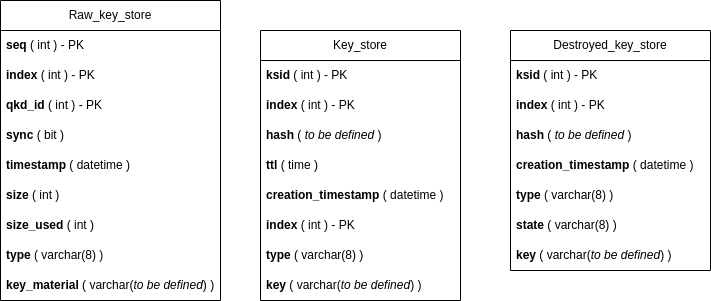
\includegraphics[width=15cm]{db.png}
	\caption{Database entity relationship diagram}
	\label{fig:dberd}
\end{figure}

As can be seen in diagram above (\autoref{fig:dberd}), the \ac{DB} is divided into three main tables. 

The \textit{Raw\_key\_store} has key material as received from the physical layer. This key material is not considered internally to be a already created key, instead will be used in the future to create keys when requested by the applications. This table is organized into the following fields:
\begin{itemize}
	\item seq (int)(PK) - Sequence number attached to the frame sent by the QKD device.
	\item index (int)(PK) - Index of the key material chunk after being split. The size of the data field in the frames sent by the QKD devices is variable, so it might be too large to or inconvenient to store it all in one entry in the \ac{DB}.
	\item qkd\_id (int)(PK) - QKD device identifier. 
	\item sync (bit) - Boolean value that tells if the key material is in sync with the peer.
	\item timestamp (datetime) - Date and time of when key material was save.
	\item size (int) - key material size in bytes.
	\item size\_used (int) - number of bytes already used.
	\item type (int) - key type. 0: classical symmetrical, 1: P.Q. symmetrical, 2: quantum symmetrical, 3/4: classical oblivious (A/X), 5/6: P.Q. oblivious (A/X), 7/8: quantum oblivious (A/X). 
	\item key\_material (varchar(4096)) - key material.
\end{itemize}

The table shall have a maximum number of rows, after the table is full new keys must be discarded. Let say that the maximum is set to one million entries, the \ac{DB} can store about 4 Gb of raw key material. Both this value and the maximum size of the key material might be changed depending on expected the key rate and the key material sent by the physical layer.

\vspace{5mm}

The \textit{Key\_store} table has the created keys. This table should have at least the following fields:
\begin{itemize}
	\item ksid (int)(PK) - Key stream id that the key is related to. For internal keys, set to the symmetric value of the id of the peer KMS which the key is shared.
	\item index (int)(PK) - index of the key in the context of the key stream (sequential).
	\item hash (tbd) - hash value or some kind of checksum used in order to check the integrity of the key with the peer \ac{KMS}.
	\item expiration\_timestamp (datetime) - Expiration date. 
	\item suspended (bit) - boolean value that tells if the key is in the suspended state.
	\item creation\_timestamp (datetime) - Timestamp of when the key was created.
	\item type (int) - Key type. Classical oblivious (A/X), 5/6: P.Q. oblivious (A/X), 7/8: quaSntum oblivious (A/X).
	\item used (bit) - Boolean value that tells if the keys was already given to the app. It's used in order for a GET\_KEY request is made without a given index and the the oldest key not provided yet should be returned is exists.  
	\item key\_material - key material. 
\end{itemize}

\vspace{5mm}

The final table related to keys is the \textit{Deleted\_key\_store} that its only purpose is to reduce the size of the \textit{Key\_store} by moving keys in the deleted state to this table.

\vspace{5mm}

Any key created has to go through its life-cycle. The states and timings are specified by NIST(NIST SP 800-57) and a summary of the standard can be found \href{https://cloud.ibm.com/docs/key-protect?topic=key-protect-key-states}{here}. The key state can be extracted from the \textit{expiration\_timestamp} and \textit{creation\_timestamp}. The only state that cannot be derived from the timestamps is the suspended mode, for that purpose the \textit{suspended} parameter in the \textit{Key\_store} table is used.

\vspace{5mm}

In terms of the mechanisms to keep the database to a certain degree clean, at least two scheduled events (scripts that run periodically) should be deployed in the \ac{DB} - one to delete old not synced keys from the \textit{Raw\_key\_store} and other to move keys to \textit{Destroyed\_key\_store} based on the timestamps.

%%%%%%%%%%%%%%%%%%%%%%%%%%%%%%%%%%%%%%	

\subsection{Key synchronization}
\label{key_synch}

The keys stored by peer \ac{KMS}s have to match, not necessarily be identical, in order to correctly providing them to the applications. A key is synchronized if both peers have received it and both are aware of that fact.

A \ac{KMS} to inform its peer of what keys it has received from the physical layer, a \textit{key\_synch} message is sent with a set of \textit{index}s of the keys received since the last message of the same type. The number of \textit{index}s in one message it may vary from KMS to KMS, as an example a \ac{KMS} with a higher key rate might have a higher number of SEQ\_ID's per message. For this process to work properly the \textit{Key\_chunk\_size} agreed on between each KMS and the respective QKD device need to be same, otherwise it's impossible to synchronize the keys using this method.

\vspace{5mm}

Each time a new key\_buffer is received by a KMS, an action will be performed based on the following criteria:
\begin{itemize}
\item current index  was mentioned in a KEY\_SYNC message sent by the peer KMS, and the number of distinct indexs was reached in order to send a KEY\_SYNC message:
	
action: send KEY\_SYNC message to peer including the last received index and store key material with sync field at 1 (true).

\item current index was not mentioned by its peer KMS’s KEY\_SYNC messages and the last notified seq is higher than the current seq:

action: discard keys

\item default:

action: store keys with sync field at 0 (false)
\end{itemize}

The sync field of a key in the \textit{raw\_key\_store} might be updated later based on the received \textit{key\_synch} messages. In order to set it to 1, both the following conditions need to be checked:
\begin{enumerate}
	\item A KEY\_SYNC message was received from the peer with the index of the key material associated with the key.
	\item The \ac{KMS} has sent a \textit{key\_synch} message notifying the peer the reception of the key material from where the key was took. 
\end{enumerate}

Not synced keys should be discarded after a high enough time period for a well functioning \ac{KMS} to send at least one \textit{key\_synch} message. The value of this time period must be configurable. The removal of keys from the \ac{DB} is made by a routine programmed in the \ac{DB} that runs periodically (see \ref{key_storage}).

%%%%%%%%%%%%%%%%%%%%%%%%%%%%%%%%%%%%%%

\subsection{Key relay}
\label{kms_key_relay}

Since the QKD devices only generate matching key material between two directly connected devices, but matching keys are required to be present at two arbitrary nodes, a process to take a key from a \ac{KMS} to other \ac{KMS} (from a node to another node) not directly connected need to be available. A QKD Key Association Link is a logical key association between two remote SD-QKD nodes, each one being of one of two types: direct, if there is a quantum channel connecting the nodes, or virtual if keys are forwarded(key relay) through multiple trusted nodes to form an end-to-end association.

The key relay process, the creation and configuration of virtual links, is managed by the SDN Controller and the key relay is performed by a set of \ac{KMS}s. The KMS / SDN Agent interaction during this process is not much specified in the standards (ETSI QKD 004 [1] and 015 [2]), though we know that each relay node is configured with the previous and next node in the path, the respective \textit{ksid} and relay method to be used. In some specific cases where there is redundant direct links between nodes, it might also specify the link for the relay. This configuration is done between the NEW\_APP and APP\_REGISTRATION requests (see \ref{kms_agent}). Those properties are used by the SDN Agent to configure the \ac{KMS}.

\vspace{5mm}

\begin{figure}[H]
	\centering
	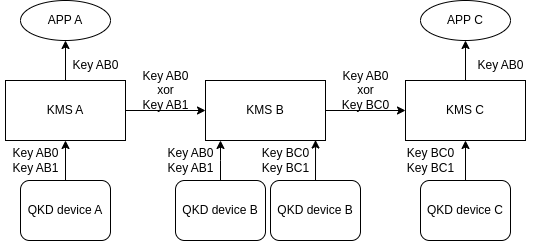
\includegraphics[width=15cm]{key_relay.png}
	\caption{Key relay process}
	\label{fig:keyrelay}
\end{figure}

The basic key relay method (see \autoref{fig:keyrelay}) is done by using \ac{OTP} performing a XOR between the key to be relayed and a key that both peer \ac{KMS}s know, this operation is done each hop. This key relay method requires all nodes to be trusted,  in some specific cases that might be a problem. In a future implementation of the system more relay method can be added and used based on the security requirements on each end-to-end connection. Some other methods can be found in ETSI QKD 014 [4] and in this paper [5].

%%%%%%%%%%%%%%%%%%%%%%%%%%%%%%%%%%%%%
\subsection{Communication between KMSs}
\label{kms_com}

The communication directly between peer \ac{KMS}s is done over a low fidelity channel used only for synchronization purposes. There's two types of massages, namely:

\begin{itemize}
	\item NEW\_KEY
		\begin{itemize}
			\item \textbf{Parameters} - Key Stream Id (Ksid), index, hash
			\item \textbf{Goal} - Establish the creation of a key.
			\item \textbf{Observations} - The peer KMS should create the key too and acknowledge it. The KMS that sends this message should only create the key after receiving the acknowledgement. If the message is not acknowledge during a valid time period (timeout defined in the QoS field in the OPEN\_CONNECT request) no key should be created. The \textit{index} field is not the index of the key to be created but the index of the raw key material from where the key will be extracted and it's optional.
		\end{itemize}
	\item NEW\_INTERNAL\_KEY
		\begin{itemize}
			\item \textbf{Parameters} - index, hash
			\item \textbf{Goal} - Establish the creation of a key to be used internally by both peer KMSs. Usually, this keys are used for authentication and integrity check of messages when communicating with each other.
		\end{itemize}
	\item KEY\_SYNC 
		\begin{itemize}
			\item \textbf{Parameters} - Received key indexs (received\_indexs)
			\item \textbf{Goal} - Notify peer of what key material it was received from the physical layer. See \ref{key_synch}.
		\end{itemize}
	\item KEY\_RELAY
		\begin{itemize}
			\item \textbf{Parameters} - Multiple encrypted keys, their respective IDs and the ID of the relay process (used to know the next hop)
			\item \textbf{Goal} - Forward keys to the next hop in the key relay process enabling key share between two not directly connected nodes. 
		\end{itemize}
\end{itemize}

%%%%%%%%%%%%%%%%%%%%%%%%%%%%%%%%%%%%%%
\subsection{Quality of service providing}
In order for the QKD network to work effectively, the SDN Controller need to be aware of some basic QoS parameters of the \ac{KMS}. The \ac{KMS} at any point can receive a request from the SDN Agent asking for the current QoS metrics, for that the \ac{KMS} has a dedicated module (QoS provider) that keeps a updated set of metrics of the current state of the system. This parameters are not specified explicitly in the specifications, but some can be extracted from some of the operations done by the SDN Controller like the proposed optimal key relay path computation algorithm. Each QoS parameter that might vary from key type to key type (e.g. key\_availability) must be provided such way that distinction can be made. For now, the QoS metrics are:

\begin{itemize}
	\item \underline{key\_availability}
	
	Total size of key material ready to be used (in bytes).
	
	\item \underline{key\_rate}	
	
	Rate at which keys are received from the QKD devices. 
	
	\item \underline{effective\_key\_rate}	
	
	Rate at which keys can be provided to an application (in bps). Does not include key that are used internally by the KMS.
	
	\item \underline{average\_key\_consuption\_per\_link}	
	
	Average key consumption (in bps). Very useful to compute optimal paths (in bps).
	
\end{itemize}

%%%%%%%%%%%%%%%%%%%%%%%%%%%%%%%%%%%%%%
\subsection{Algorithm security}
To assure \ac{ITS} of the system as a whole, every module need to use \ac{ITS} algorithms to promise security against an adversary with unbound computational power. 

\subsubsection{Authentication and integrity}
Can be achieved by using a \ac{MAC}, such as UMAC or Poly1305. Both the transmitter and the receiver have a shared secret, used by the first to create the \ac{MAC} and by the other to verify the authenticity of the sender and the integrity of the message. This must be used in all communication where is possible to have shared keys, such between KMSs where it can take an advantage from QKD. But in order to assure both this aspect in a communication such as between the KMS and a secure app the use of asymmetrical algorithms would be perfect to bypass the QKD, but classical \ac{KEM} is not IT secure. The use of post-quantum and hybrid algorithms could be used to authenticate and share a keys between them. There's a very limited amount of \ac{ITS} post-quantum algorithms, right now being advised to use hybrid algorithms instead. The use of certificates would simplify authentication and authorization allowing all entities in the system to identify themselves and others.

\subsubsection{Encryption}
Encryption is most importantly used in the communication between KMSs since all data is transmitted over the black network. Idealizing the use of QKD shared keys, the encryption of data can be as simple as a XOR, that is IT secure as long a different key is always used and its size it's equal to the size of the data to encrypt.


%%%%%%%%%%%%%%%%%%%%%%%%%%%%%%%%%%%%%%

\subsection{Sequence Diagrams}
\label{seq_diagrams}

\section{Two node basic scenario}

In this scenario we consider a two nodes, Node A and Node B, directly connected in two distinct sites. App A and App B want to communicate, in order to get keys they connect to their respective \ac{KMS}. This scenario can be considered one the most simple, representing the backbone of the system.

\begin{figure}[H]
	\centering
	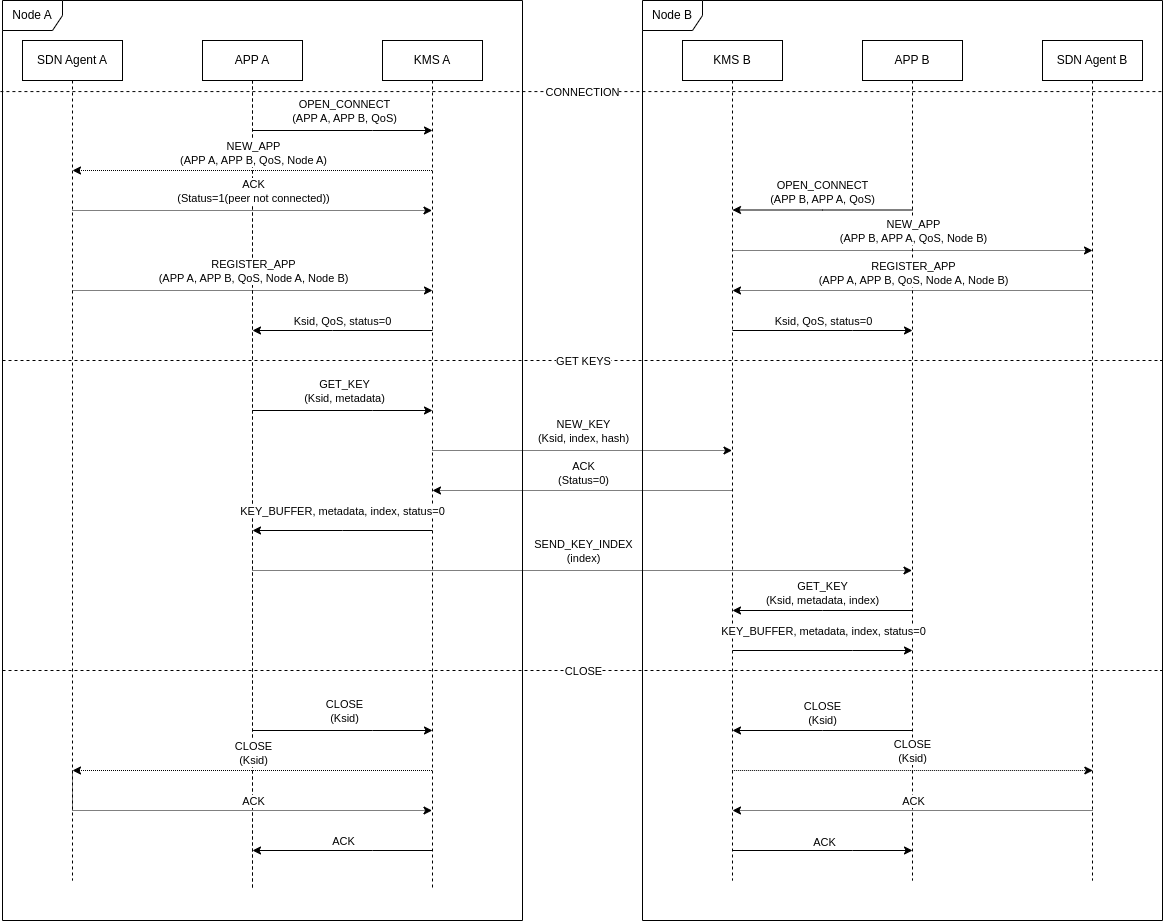
\includegraphics[width=15cm]{seq_diagram_0.png}
	\caption{Sequence diagram for a basic scenario with two directly connected nodes.}
	\label{fig:seq0}
\end{figure}

The workflow description associated with the sequence diagram (\autoref{fig:seq0}) is as follows:
\begin{itemize}
 	\item In node A, APP A makes an OPEN\_CONNECT request in order to create a connection to the \ac{KMS}. The goal of APP A is to communicate to APP B and vice-versa, so the \textit{source} is APP A, the \textit{destiny} is APP. 
 	\item \ac{KMS} A agrees on the QoS parameters proposed by the APP A. In order to know the location of APP B, sends a NEW\_APP request to the SDN Agent A.
 	\item In the instant that the SDN Controller is informed of the connection of APP A to KMS A in node A, APP B is to yet connected, so the SDN Agent acknowledges the NEW\_APP request  with a status code informing that the peer app is not connected.
 	\item In node B, APP B makes a OPEN\_CONNECT and the SDN Controller is notified via SDN Agent B.
 	\item With both applications connected the SDN Controller creates a global unique \textit{ksid} and, since Node A and Node B are directly connected, simply informs both \ac{KMS}s via the SDN Agents of the \textit{ksid} and \textit{qkdn\_id} of both nodes.
 	\item Both \ac{KMS} answer to the OPEN\_CONNECT request made previously by indicating the QoS and \textit{ksid} inherent to the connection.
 	\item App A makes a GET\_KEY request, giving the ksid and the metadata field only with the Metadata\_size that dictates the maximum size of the metadata buffer.
 	\item KMS A notifies KMS B of the creation of a new key for a specific \textit{ksid}. The \textit{index} field is not the index of the key to be created but the index of the raw key material from where the key will be extracted and it's optional. The \textit{hash} field is used for KMS B to check the integrity of the key that will be created. KMS B creates the key and acknowledges with a successful status code.
 	\item KMS A creates the key too and sends it to APP A alongside its metadata and index. The metadata might include creation and expiration timestamps and key type.
 	\item APP B receives a key index (how it's sent is out of the scope of the \ac{KMS}) and requests the key to \ac{KMS} B that responds with a key matching the one received previously by APP A. It's important to note that the result of this GET\_KEY request would be the same if no index would be provided by the application, since the oldest active key attached to this key stream is the one withe that index.
 	\item Both applications send a CLOSE request to their respective \ac{KMS}s to terminate the given key stream. The SDN Agents (consequently the SDN Controller too) are notified. Finally, both applications CLOSE request is acknowledge.
 	
\end{itemize}

\pagebreak

%%%%%%%%%%%%%%%%%%%%%%%%%%%%%%%%%%%%%%
% Acronyms
%%%%%%%%%%%%%%%%%%%%%%%%%%%%%%%%%%%%%%
\clearpage
\subsection*{Acronyms}\label{sec:acronyms}
\begin{acronym}[TDMA]
	\acro{KML}[KML]{Key Management Layer}
	\acro{KMS}[KMS]{Key Management System}
	\acro{KSID}[KSID]{Key Stream Id}
	\acro{SDN}[SDN]{Software Defined Network}
	\acro{RNG}[RNG]{Random Number Generator}
	\acro{DB}[DB]{Database}
	\acro{OTP}[OTP]{One Time Pad}
	\acro{ITS}[ITS]{Information-Theoretic Security}
	\acro{MAC}[MAC]{Message Authentication Code}
	\acro{KEM}[KEM]{Key Encapsulation Mechanism}
\end{acronym}
\pagebreak 


%%%%%%%%%%%%%%%%%%%%%%%%%%%%%%%%%%%%%%
% References
%%%%%%%%%%%%%%%%%%%%%%%%%%%%%%%%%%%%%%

% bibliographic references for the section 
\clearpage
\subsection{References}

\begin{enumerate}
	\item ETSI GS QKD 004, V2.1.1, 2020-08
	\item ETSI GS QKD 015, V2.1.1, 2022-04
	\item Discretion D3.1 SDN Preliminary Design Report, 2023
	\item ETSI GS QKD 014, V1.1.1, 2019-02
	\item Multiple stochastic paths scheme on partially-trusted relay quantum key distribution network, Hao, 2009
\end{enumerate}

\clearpage
\printbibliography[heading=subbibliography]
\end{refsection}
\addcontentsline{toc}{subsection}{Bibliography}
\cleardoublepage
